\documentclass[submitting]{nst}

\usepackage{subfigure,dcolumn}
\usepackage{epstopdf}
\usepackage{mhchem}
\usepackage{upgreek}
\usepackage{subfigure}
\usepackage{physics}
\usepackage{listings}
\usepackage{dcolumn}

\begin{document}

%\title{Quasi-frozen spin for both deutron and proton beam at EDM storage ring and axion search}
\title{Quasi-frozen spin for both deutron and proton beam\\ at periodic EDM storage ring lattice and axion search}
%\thanks{Supported by the Program for Science \& Technology Innovation Talents in Universities of Henan Province (No.~13HASTIT046) and the Young Teacher Project in Henan Normal University}

\author{Kolokolchikov S. D.}
\email[Corresponding author, ]{sergey.bell13@gmail.com}
\affiliation{Institute for Nuclear Research of the Russian Academy of Sciences, Moscow 117312, Russia}

\author{Senichev Yu. V.}
\affiliation{Institute for Nuclear Research of the Russian Academy of Sciences, Moscow 117312, Russia}

\author{Aksentyev A. E.}
\affiliation{Institute for Nuclear Research of the Russian Academy of Sciences, Moscow 117312, Russia}
\affiliation{National Research Nuclear University MEPhI, Moscow 115409, Russia}

\author{Melnikov A. A.}
\affiliation{Institute for Nuclear Research of the Russian Academy of Sciences, Moscow 117312, Russia}
\affiliation{Landau Institute for Theoretical Physics, Chernogolovka 142432, Russia}

\author{Palamarchuk P. I.}
\affiliation{National Research Nuclear University MEPhI, Moscow 115409, Russia}

\begin{abstract}
A novel experimental setup with spatially separated magnetic and electrostatic fields is proposed for studying the electric dipole moment (EDM) of deuterons and protons. The design leverages Wien filters to achieve precise measurements under "quasi-frozen" spin conditions, demonstrating adaptability to existing facilities for research at higher energy levels and advanced axion search.
\end{abstract}

\keywords{Electric dipole moment, Quasi-frozen spin, Wien filter, Electrostatic deflector, Axion}

\maketitle

\section{Introduction}\label{sec.I}
\par The investigation of the electric dipole moment (EDM) of fundamental particles, such as protons and deuterons, constitutes a critical endeavor in contemporary physics. EDM offers an unparalleled opportunity to probe CP violation and validate theoretical models that describe particle interactions beyond the framework of the Standard Model \cite{EDM}. For charged particles, the precise measurement of EDM necessitates the use of accelerators and the development of novel methodologies and technologies, requiring the adaptation of existing accelerator facilities to meet these experimental demands.

\par This paper explores a versatile structure characterized by spatially segregated magnetic and electrostatic fields, uniquely designed to facilitate the study of EDM in both deuterons and protons. A notable feature of this structure is its ability to support experiments for both types of particles, thereby enhancing its applicability and efficiency. Special emphasis is placed on the utilization of Wien filters or electrostatic deflectors with kicker to compensate for the magnetic dipole moment (MDM) and establish conditions conducive to a "quasi-frozen" spin. The analysis elucidates how such a structure can be adapted for facilities not originally intended for such experiments and explores its potential for advancing research at higher energy levels. An advanced research on searching axion or axion-particles can be also successfully done at QFS structure.
 
\section{Quasi-frozen spin at periodic lattice}\label{sec.II}

\par For an ensemble of particles, the spin can be described as a classical vector and its dynamics evaluated in external electromagnetic fields using the Thomas-Bargmann-Michel-Telegdi (T-BMT) equation \cite{TBMT}

\begin{equation}
	\begin{aligned}
		\dv{\vec{\mathrm{S}}}{t} = & \left(\vec{\Omega}_{\text{MDM}}+\vec{\Omega}_{\text{EDM}}\right)\times\vec{\mathrm{S}}, \\
		\vec{\Omega}_{\text{MDM}}  = & - \frac{q}{m \gamma}\left\{(\gamma G+1) \vec{\mathrm{B}}_{\perp}+(G+1) \vec{\mathrm{B}}_{\|}-\right. \\
								     & \left.-\left(\gamma G+\frac{\gamma}{\gamma+1}\right) \frac{\vec{\beta} \times \vec{\mathrm{E}}}{c}\right\}, \\
		\vec{\Omega}_{\text{EDM}}  = & - \frac{q \eta}{2 m}\left(\vec{\beta} \times \vec{\mathrm{B}}+\frac{\vec{\mathrm{E}}}{c}\right), \quad G=\frac{g-2}{2},
	\end{aligned}
	\label{eq:T-BMT}
\end{equation}

\noindent where $\vec{\Omega}_{\text{MDM}}, \vec{\Omega}_{\text{EDM}}$ -- are the angular speed of rotation due to magnetic and electric dipole moment, $\vec{\mathrm{E}}, \vec{\mathrm{B}} = \vec{\mathrm{B}}_{\perp} + \vec{\mathrm{B}}_{\|}$ -- external magnetic and electric field. $m, q$ — mass and charge of a particle, $\gamma$ is Lorenz factor. Dimensionless $\eta$ factor is connected
to the EDM value $d$ and spin $s$ of a particle: $d = \frac{\eta g}{2mc}s$. 

\par For EDM measurements, it is first necessary to compensate for MDM-effect. The simplest approach, initially proposed at BNL \cite{AGS}, involves fully compensating the magnetic field with an electric field aligned along the momentum. This method requires the use of elements that incorporate both magnetic and electric fields, and the lattice must be specifically designed and operated for EDM research.
\par An alternative approach is the quasi-frozen spin concept, based on the principle of sequential spin compensation \cite{QFS}. In this scenario, the EDM measurement slightly deviates from the frozen spin condition, as given by $S_{\text{EDM}}=1-\frac{\alpha^2}{4} \simeq 0.998$, where $\alpha$ represents the small angle associated with the MDM-effect.

\subsection{Relative spin motion at QFS}    

\par Let us introduce the concept of QFS by examining orbital and spin rotation in a generalized framework. This approach is based on the dynamics governed by the Lorentz force for orbital motion and T-BMT equation for spin precession. It is essential to first ensure that the orbital trajectory remains unaltered, maintaining a closed orbit configuration.

\begin{equation}
	\Phi_p^{\textrm{arc}}+\Phi_{p}^{\textrm{comp}}=\frac{2\pi}{N}\ \ \
	\label{eq:QFS_orbital}
\end{equation}

\noindent where index $p$ states for momentum, $\Phi_p^{\textrm{arc}}$ and $\Phi_{p}^{\textrm{comp}}$ -- total momentum rotation in arc and spin compensator element, $N$ is the lattice periodicity. To facilitate a lattice suitable for both EDM studies and high-energy researches, it is essential to employ a pure magnetic arc with a guiding field, given the limitations of achievable electric field strengths. This way a corresponding spin compensator should be implemented and not violate orbit at all. It can be formulated as $\Phi_p^{\textrm{arc}} = \frac{2\pi}{N}$, then $\Phi_{p}^{\textrm{comp}} = 0$. In order to compensate Lorenz force, the spin compensator must utilize both magnetic and electric fields. From the eq. \ref{eq:QFS_orbital} for spin compensation element with both magnetic and electric field

\begin{equation}
	\Phi_{p\textrm{B}}^{\textrm{comp}}+{\Phi}_{p\textrm{E}}^{\textrm{comp}} = 0\ \ \ 
\end{equation}

\noindent where $\Phi_{p\textrm{B}}^{\textrm{comp}}$ and ${\Phi}_{p\textrm{E}}^{\textrm{comp}}$ -- total momentum rotation in magnetic and electric field at spin compensator. From T-BMT equation \ref{eq:T-BMT} it can be seen that maximum effectiveness on spin electric field then it is radial to the momentum. Moreover, the momentum rotation has also the maximum value for radial electric force, which means the most effectiveness for applied field

\begin{equation}
	\vec{\Omega}_{p\mathrm{E}}^{\text{max}} = \vec{\Omega}_{p\mathrm{E}_{\perp}}=\frac{q}{m \gamma} \frac{\vec{\beta} \times \vec{\mathrm{E}}_{\perp}}{c \beta^2}
\end{equation}

\par The second condition is to compensate MDM spin rotation in one period of the ring 

\begin{equation}
	\Phi_s^{\textrm{arc}}+\Phi_{s}^{\textrm{comp}}=0,
	\label{eq:QFS_spin}
\end{equation}

\noindent where $\Phi_s^{\textrm{arc}}$ and $\Phi_{s}^{\textrm{comp}}$ -- total spin rotation in arc and spin compensator. The ratio of spin rotation relative to orbital one as follows given by spin-tune in magnetic and electric field

\begin{equation}
	\nu_{\mathrm{B}_{\perp}} = \gamma G, \quad \nu_{\mathrm{E}} = \gamma \beta^2 \left(G-\frac{1}{\gamma^{2}-1}\right).
	\label{eq:spin-tine}
\end{equation} 

 \noindent So, compensation occurs due to the fundamental difference between spin rotation in a magnetic and electric field. And the coupling equations for pure magnetic arc $\Phi_{s}^{\text{arc}} = \nu_{\mathrm{B}_{\perp}}\Phi_{p}^{\text{arc}}$ and magnetic $\Phi_{s\mathrm{B}}^{\text{comp}} = \nu_{\mathrm{B}_{\perp}}\Phi_{p\mathrm{B}}^{\text{comp}}$ and electrical $\Phi_{s\mathrm{E}}^{\text{comp}} = \nu_{\mathrm{E}}\Phi_{p\mathrm{E}}^{\text{comp}}$ in spin compensator ,. Than for eq. \ref{eq:QFS_spin}
 
 \begin{equation}
 	\begin{aligned}
 	\nu_{\mathrm{B}_{\perp}}\Phi_{p}^{\text{arc}} +
 	\left(\nu_{\mathrm{B}_{\perp}}\Phi_{p\mathrm{B}}^{\text{comp}} +
 	\nu_{\mathrm{E}}\Phi_{p\mathrm{E}}^{\text{comp}} \right) & = \\
 	= \nu_{\mathrm{B}_{\perp}} \left( 
 	\Phi_{p}^{\text{arc}} +
 	\Phi_{p\mathrm{B}}^{\text{comp}} \right) +
 	\nu_{\mathrm{E}}\Phi_{p\mathrm{E}}^{\text{comp}}  & = 0.
 	\label{eq:deflection}
 	\end{aligned}
 \end{equation}
  
 \par Finally, from first and second condition can be received for rotation via magnetic or electric field in spin compensator element

\begin{equation}
	\Phi_{p\mathrm{E}}^{\textrm{comp}} = - \Phi_{p\mathrm{B}}^{\textrm{comp}} = {\Phi}_{p}^{\text{arc}}\frac{\gamma^2 G}{G+1} =\frac{2\pi}{N}\frac{\gamma^2 G}{G+1}.
	\label{eq:deflection}
\end{equation}

\noindent No mention was made of the physical structure of the compensation element, only of the integral features of the presented field components.

\subsection{Spin compensation element length}

Spin compensation element length can be calculated for magnetic and electric field

\begin{equation}
	L = \Phi_{p\mathrm{B}}^{\text{comp}}R_{\mathrm{B}} = \Phi_{p\mathrm{E}}^{\text{comp}}R_{\mathrm{E}}
	\label{eq:length}
\end{equation}

\noindent where $R_{\mathrm{B}}, R_{\mathrm{E}}$ -- radius of magnetic and electric field. In general, total radius for element with combined magnetic and electric fields can be find as

\begin{equation}
	\frac{1}{R} = \frac{1}{R_{\mathrm{B}}}+\frac{1}{R_{\mathrm{E}}}, \quad R_{\mathrm{B}}=\frac{\mathrm{B}\rho}{\mathrm{B}}, \quad R_{\mathrm{E}}=\frac{\kappa}{\mathrm{E}}    
	\label{eq:total_radius}
\end{equation}

\noindent where $\mathrm{B}\rho = \cfrac{p_{0}}{e}$ -- magnetic rigidity, $p_{0} = \gamma m\beta c$, $\kappa = \cfrac{p_{0}\beta c}{e}$ -- electrical rigidity. If we consider no orbital distortion in total, Lorentz force should be zero, so $R=0$ and $R_{\mathrm{B}} = -R_{\mathrm{E}}$.

The limitation on the strength of the electric field is much more significant than in the case of a magnetic field. According to the eqs. \ref{eq:deflection} and \ref{eq:length} can be received the length of compensator element per one period

\begin{equation}
	\begin{aligned}
	L_{\text{min}} = \Phi_{p\mathrm{E}}^{\text{comp}}R_{\mathrm{E}} & = 
	\frac{2\pi}{N}\frac{\gamma^2 G}{G+1}\frac{\kappa}{\mathrm{E}_{\text{max}}} = \\
	& = \frac{2\pi}{N}\frac{G}{G+1}\frac{mc^2}{e}\frac{\gamma(\gamma^2-1)}{\mathrm{E}_{\text{max}}}
	\label{eq:length_min}
	\end{aligned}
\end{equation}

\noindent where $\mathrm{E}_{\text{max}}$ -- maximum of electric field, that limit the minimal achievable length regardless the researched particle. For total length $L=L_{\text{min}}^{\text{total}} = N\cdot L_{\text{min}}$ and is independent from number of periods. Maximum achievable electric field values 10-13 V/m \cite{wien}, this corresponds to a magnetic field of the order of 70-90 mT accordingly, it will be used later for evaluation.

\section{Features of Proton and deuteron}\label{sec.III}

\subsection{Dependence on beam parameters}

\par To effectively analyze spin dynamics, it is essential to maximize the analyzing power of the polarimeter. Thus, the beam energy plays a critical role in achieving sufficient experimental statistics for this purpose. The maximum analyzing capability of the polarimeter is reached at a beam energy of 270 MeV \cite{Pol}. 

\par Additionally, orbital and spin dynamics vary among different types of particles. First, the mass-to-charge ratio of deuterons is twice that of protons. Second, the anomalous magnetic moments for protons and deuterons are notably different: $G_{\text{p}} = 1.79$  for protons and $G_{\text{d}} = -0.14$ for deuterons. These differences necessitate tailored approaches for each particle type when designing experiments (Table \ref{tab:particles}) and analyzing results.

\begin{table}[!htb]
	\caption{Particles and experiment parameters.}
	\label{tab:particles}
	\begin{tabular*}{8cm} {@{\extracolsep{\fill} } lccccc}
		\toprule
		Particle & $A/Z$ & $G$     & $\gamma_{\text{exp}}$ & $E_{\text{exp}}$, MeV per nucleon  & $L$, m \\
		\midrule
		Deuteron $\text{d}$ & $2$   & $-0.14$ & $1.144$  & $135$ & $53$ \\
		Proton $\text{p}$ & $1$   & $1.79$  & $1.289$ & $270$ & $247$ \\
		  &    &   & $1.078$ & $73$ & $53$ \\
		\bottomrule
	\end{tabular*}
\end{table}

% TODO: \usepackage{graphicx} required
\begin{figure} [h!]
	\centering
	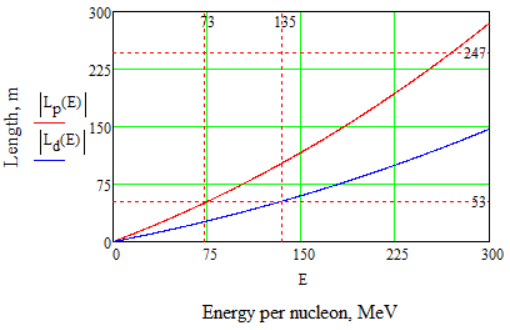
\includegraphics[width=0.95\linewidth]{total_length}
	\caption{Total length of spin compensator needed to make QFS lattice for deuteron and proton.}
	\label{fig:totallength}
\end{figure}

\par In a magnetic field, according to eq.\ref{eq:spin-tine} the direction of rotation depends solely on the sign of the anomalous magnetic moment and is independent of energy. However, the magnitude of the relative rotation is influenced by both the energy and the strength of the magnetic field. For protons this effect is so important as spin rotation per arc should be limited $\gamma G \cdot \Phi_{p}^{\text{arc}} < \pi/2$ to save an ability for EDM storage. And usage of periodic structures can save the idea of measuring proton EDM with QFS lattice, should be at least $N=8$ and greater. 

\par In electrostatic fields, the behavior of protons and deuterons is further complicated by their distinct interactions with the field. For protons, the direction of spin rotation can depend on the energy, particularly around the "magic energy" where $\gamma_{\text{mag}} = \sqrt{\cfrac{G_{\text{p}}+1}{G_{\text{p}}}} = 1.248$ ($240$ MeV). At any way the influence on proton is much lower than for deuterons. For deuterons, however, there is no equivalent "magic energy," and their spin rotation behavior remains consistent across energy levels. (Fig. \ref{fig:spin-tune})

% TODO: \usepackage{graphicx} required
\begin{figure} [h!]
	\centering
	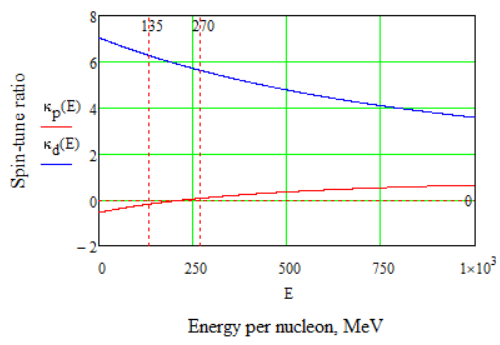
\includegraphics[width=0.95\linewidth]{spin-tune_ratio}
	\caption{Spin-tune ratio $\kappa = \cfrac{\nu_{\mathrm{B}_{\perp}}}{\nu_{\mathrm{E}}}$ for deuteron and proton.}
	\label{fig:spin-tune}
\end{figure}


\par These fundamental differences lead to several important consequences for lattice construction. Specifically, modifications are necessary to accommodate the study of both particle types. According to eq. \ref{eq:deflection} the sign of rotation for proton and deuteron differs. This shows the necessity of spin compensator rotation by $\pi$ along the longitudinal axis. Additionally, the minimal achievable spin compensator length as given by eq. \ref{eq:length_min}), is longer for proton than for deuterons at optimal polarimeter energy. This discrepancy can be addressed by lowering the experimental energy for protons. At a spin compensator length equivalent to that used for deuterons, the proton energy should be reduced to 73 MeV, the analyzing power decreases by a factor of 2-3, which is useful for methodological refinement but insufficient for statistical validation. Two viable approaches for arranging additional EM-fields are the implementation of a Wien filter or an electrostatic deflector with a kicker.

\subsection{Wien filter}

\par The Wien filter is a crucial tool in particle accelerators, designed to manipulate spin dynamics without altering the orbital trajectory of particles by utilizing perpendicular electric and magnetic fields that cancel each other out, resulting in zero net Lorentz force. This configuration allows particles to move in a straight line while enabling precise control over their spin orientation, making it ideal for experiments requiring spin manipulation. The filter's design, ensures no net deflection along the beamline, minimizing additional space requirements in the ring's straight sections and allowing for a classical sequential arrangement of ring elements. 

Its adaptability is evident in its use for both deuterons and protons; for deuterons, it can be employed directly at optimal energies, while for protons, it must be rotated by $\pi$ along the longitudinal axis and used at lower energies (Fig. \ref{fig:wien-filter}). This flexibility facilitates the development of methodologies for studying spin dynamics across different particle types, enhancing experimental strategies. Overall, the Wien filter's ability to control particle spin without disrupting orbital paths makes it an invaluable component in advanced accelerator experiments.

% TODO: \usepackage{graphicx} required
\begin{figure} [h!]
	\centering
	a. Deuteron\\
	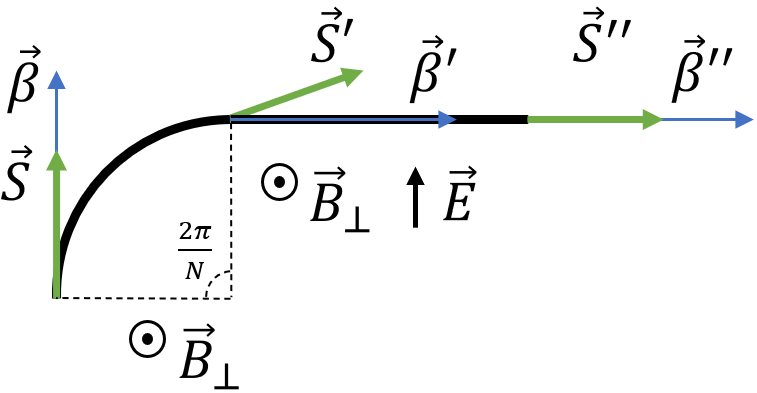
\includegraphics[width=0.8\linewidth]{wien-filter_deuteron}\\
	b. Proton\\
	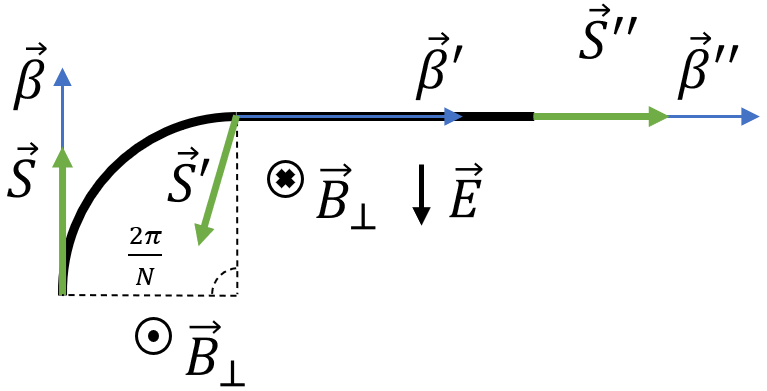
\includegraphics[width=0.8\linewidth]{wien-filter_proton}
	\caption{One period conceptual scheme of QFS lattice with Wien filters for a. deuterons, b. protons.}
	\label{fig:wien-filter}
\end{figure}

\subsection{Electrostatic deflector with kicker}

\par Pure electrostatic deflector designed to manipulate particle trajectories and spin dynamics by creating a radial electric field with non-zero curvature. Unlike the Wien filter, this deflector requires an additional kicker to compensate for orbital deviations, which increases the overall length of the compensator. This setup is particularly useful for creating bypass sections in addition to native straight sections, allowing for flexible experimental configurations (Fig. \ref{fig:el-defdeuteron}). But it should be considered distance between the spatial assignment of equipment to enable option with independent section. However, it necessitates careful consideration of the spatial arrangement of equipment to enable independent section operation. A key challenge is that each type of particle requires a different curvature, which must be determined at the outset of lattice design. Despite these complexities, the electrostatic deflector with kicker offers a robust solution for controlling particle spin and trajectory.

% TODO: \usepackage{graphicx} required
\begin{figure} [!h]
	\centering
	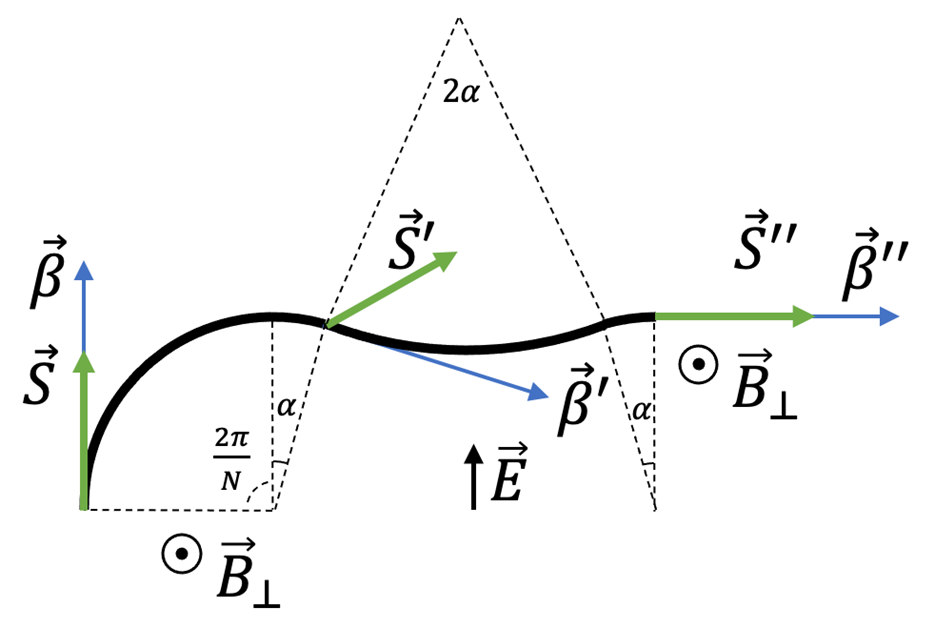
\includegraphics[width=0.8\linewidth]{el-def_deuteron}
	\caption{One period conceptual scheme of QFS lattice with electrostatic deflector and kicker for deuterons.}
	\label{fig:el-defdeuteron}
\end{figure}


\section{Further researches}\label{sec.IV}	

\subsection{Research at higher energy level}

\par Currently, the proposed energy requirements for EDM studies are set at 270 MeV and lower, but specific conclusions regarding arc rotation have yet to be drawn. The primary condition is to achieve a momentum rotation at a specific angle $\Phi_p^{\textrm{arc}}$ with a corresponding $\Phi_s^{\textrm{arc}}$ for spin. This can be accomplished by carefully selecting the magnetic field integral to ensure precise alignment of momentum and spin dynamics. To maximize effectiveness, the magnetic field should be as strong as possible to minimize the effective arc length, considering the unique features of the lattice design. This approach not only optimizes studies at current energy levels but also opens the possibility for research at higher energies, potentially reaching several GeV. The versatility of the quasi-frozen spin (QFS) structure allows it to be implemented in various lattice designs, including existing accelerator rings, thereby facilitating advanced studies at elevated energy levels.

\subsection{Axion search}

\par The QFS lattice in storage rings presents a unique opportunity for axion searches by utilizing the spin of polarized particles as highly sensitive detectors. Axions, initially proposed to resolve the strong CP problem in QCD, are potential candidates for dark matter. The axion halo interacts with spin as a pseudo-magnetic field, effectively acting as a solenoid and allowing the scan frequency to reach resonance. By varying the beam energy, researchers can adjust the spin precession frequency to scan for axion signals. The hybrid nature of the QFS lattice, which combines electric and magnetic bending, broadens the range of detectable axion masses. This setup is particularly advantageous for probing small mass axions, as it allows operation at fixed beam energies with optimized polarimetry and reduced decoherence effects.

\par By monitoring the buildup of vertical polarization from an initially horizontal state, researchers can detect resonant interactions with axions, even in the presence of short spin coherence times. This methodology is adaptable to both proton and deuteron beams, opening new avenues for axion searches in existing and future storage ring facilities, including COSY \cite{COSY} and the proposed PTR \cite{PTR} and NICA \cite{Axion}. At the COSY ring, an experiment utilized an RF Wien Filter, which acted as an additional field to induce a resonant spin flip at a certain frequency. Additionally, CERN has proposed the Prototype ring (PTR), where the concept of frozen spin will be implemented, further advancing the capabilities for axion detection.

\section{Summary} \label{sec.V}

\par This article presents the implementation of a "quasi-frozen" spin structure for a periodic lattice to study the Electric Dipole Moment of charged light particles. The design achieves precise spin compensation of MDM-effect per one period by employing elements with matched curvatures for electric and magnetic fields, allowing for effective spin manipulation. Wien filters, which do not cause beam deflection, and electrostatic deflectors, which enable bypass creation, are integral to this flexibility. An expression for the  optimal spin compensator length is derived. Notably, the setup allows for the investigation of proton EDM using the same ring as for deuterons, simply by rotating the spin compensator by 180 degrees and operating at reduced energy.

\par The study demonstrates the versatility of the quasi-frozen spin lattice, which can be adapted for multiple purposes, including higher-energy research within existing facilities and, additionally, the unique capability of the structure to axion searches, what underscores its significance in advancing particle physics research.

\section*{ACKNOWLEDGMENTS}

\par A support of thus study by the Russian Science Foundation grant ??-??-????? is acknowledged.

\begin{thebibliography} {99}
	\bibitem{EDM} M.Pospelov, A.Ritz, Electric dipole moments as probes of new physics. DOI: 10.1016/j.aop.2005.04.002
	\bibitem{TBMT} Bargmann, V. and Michel, Louis and Telegdi, V. L., Precession of the Polarization of Particles Moving in a Homogeneous Electromagnetic Field. https://doi.org/10.1103/PhysRevLett.2.435
	\bibitem{AGS} Anastassopoulos, D. and others, AGS proposal: Search for a permanent electric dipolemoment of the deuteron nucleus at the $10^{-29}$ $e$ cm level. 
	\bibitem{QFS} Yu.Senichev et al., Investigation of Lattice for Deuteron EDM Ring. DOI: 10.18429/JACoW-ICAP2015-MODBC4
	\bibitem{wien} Aggarwal, A. and Magiera, A., Controlling Systematic Uncertainties in Search for an EDM in the Storage Ring. DOI:  10.5506/APhysPolB.51.373
	\bibitem{Pol} M. W. Mcnaughton el al., THE P C ANALYZING POWER BETWEEN 100-MEV AND 750-MEV. DOI: 10.1016/0168-9002(85)90595-9
	\bibitem{COSY} S. Karanth et al., First Search for Axionlike Particles in a Storage Ring Using a Polarized Deuteron Beam. DOI: https://doi.org/10.1103/PhysRevX.13.031004
	\bibitem{Axion} Nikolaev, N.N. Spin of Protons in NICA and PTR Storage Rings as an Axion Antenna. Jetp Lett. 115, 639–643 (2022). https://doi.org/10.1134/S0021364022600653
	\bibitem{PTR} R. Talman, J.Talman, Predominantly electric storage ring with nuclear spin control capability. DOI 10.1088/1748-0221/19/11/P11017

%\bibitem{b1}	M. Huang, Z. Chen, S. Kowalski et al., Isobaric yield ratios and the symmetry energy in heavy-ion reactions near the Fermi energy. Phys. Rev. C {\bf 81}, 044620 (2010).   \href{http://dx.doi.org/10.1103/PhysRevC.81.044620}{doi: 10.1103/PhysRevC.81.044620}
%\bibitem{b2}	M. Huang, A. Bonasera, Z. Chen et al., Isospin dependence of the nuclear equation of state near the critical point. Phys. Rev. C {\bf 81}, 044618 (2010).   \href{http://dx.doi.org/10.1103/PhysRevC.81.044618}{doi: 10.1103/PhysRevC.81.044618}

\end{thebibliography}

\end{document}

